\documentclass{article}
\usepackage[utf8]{inputenc}
\usepackage[letterpaper,left=2cm, right=2cm, top=2.5cm, bottom=2.5cm]{geometry}
\usepackage{fancyhdr}
%%%%%%%%%%%%%%%%%%%%%%%%%%%%%%%%%%%%%%%%%%%%%%%%%%%%%%%%%%%%%%
\usepackage{amssymb}
\usepackage{amsmath}
\usepackage{rotating}
\usepackage{graphicx}
\usepackage{wrapfig}
\usepackage{subfigure}
\usepackage{subcaption}
\usepackage[mathscr]{euscript}
\usepackage[dvipsnames,svgnames,table]{xcolor}
\usepackage{multicol}
\usepackage{multirow}
\usepackage{physics}
\usepackage[version=4]{mhchem}
\usepackage[spanish,es-nodecimaldot,es-tabla]{babel}
\usepackage{parskip}
\usepackage{hyperref}
\usepackage{apacite}
\usepackage{etoolbox}
\usepackage{tcolorbox}
\tcbuselibrary{theorems}
%%%%%%%%%%%%%%%%%%%%%%%%%%%%%%%%%%%%%%%%%%%%%%%%%%%%%%%%%%%%%%
%\input{definitions}
%\input{qmdef}
\newcommand{\be}{\begin{equation*}}
\newcommand{\ee}{\end{equation*}}
\newcommand{\ble}[1]{\begin{equation} \label{#1}}
\newcommand{\bae}{\begin{eqnarray}}
\newcommand{\eae}{\end{eqnarray}}
\newcommand{\sint}{\sin{\theta}}
\newcommand{\cost}{\cos{\theta}}
\newcommand{\pl}{\left(}
\newcommand{\pr}{\right)}
\newcommand{\kl}{\left[}
\newcommand{\kr}{\right]}
\newcommand{\ii}{\int_{-\infty}^\infty}
\providecommand{\abs}[1]{\lvert#1\rvert}
\providecommand{\norm}[1]{\lVert#1\rVert}
\newcommand{\pa}{\vspace{2mm}}
\definecolor{Grayo}{RGB}{72, 72, 72}
\definecolor{Graya}{RGB}{158, 158, 158}
%%%%%%%%%%%%%%%%%%%%%%%%%%%%%%%%%%%%%%%%%%%%%%%%%%%%%%%%%%%%%%

\begin{document}

\centerline{\Large \textbf{\textcolor{Grayo}{Guía Planeación I}}}
\vspace{2mm}
\centerline{\large \textsc{Christopher López Ruiz}}

\vspace{-10pt}

\begin{center}
\line(1,0){480}
\end{center}

%%%%%%%%%%%%%%%%%%%%%%%%%%%%%%%%%%%%%%%%%%%%%%%%%%%%%
%%%%                                                               Problemas                                                                %%%%
%%%%%%%%%%%%%%%%%%%%%%%%%%%%%%%%%%%%%%%%%%%%%%%%%%%%%

%%%%%%%%%%%%%%%%%%%%%%%%%%%%%%%%%%%%%%%%%%%%%%%%%%%%%

\vspace{3pt}
%%%%%%%%%%%%%%%%%%%%%%%  PROBLEMA 1  %%%%%%%%%%%%%%%%%%%%%%
%%%%%%%%%%%%%%%%%%%%%%%%%%%%%%%%%%%%%%%%%%%%%%%%%%%%%
%

\section*{AP-PA}

\begin{figure}[!h]
    \centering
    \begin{minipage}[t]{0.5\linewidth}
        \centering
        \begin{tcolorbox}[colback=gray!25!white, colframe=gray, title=\textbf{Resumen}, center title]
            \begin{itemize}
                \item sdf
            \end{itemize}
        \end{tcolorbox}
    \end{minipage}%
    \hfill
    \begin{minipage}[t]{0.5\linewidth}
        \centering
        \includegraphics[width=0.5\linewidth]{APPA.pdf}
        \caption{Distribución campos AP-PA.}
        \label{APPA}
    \end{minipage}
\end{figure}

\subsection*{Preinspección}

Abrir estructuras, visualizar el origen de la CT de simulación en el corte axial, revisar la orientación del paciente en la visualización 3D e identificar el PTV de interés.

\subsection*{Nuevo Plan}

Se inserta una nueva etapa de tratamiento y, posteriormente, en esta etapa se añade un nuevo plan con el PTV de referencia. Seleccionar tipo de tratamiento, dosis por fracción, número de fracciones, equipo, posición del paciente y energía del LINAC.

\subsection*{Añadir campos y redondear}

Automáticamente se crea un campo con un ángulo de $\mathbf{0^{\circ}}$. En la pestaña de campos en la parte inferior de la pantalla se identifica el tamaño de campo (\textit{x, y, z}) y se modifica, si es necesario, los valores predeterminados redondeando a un paso mínimo de 5 decimales. Una vez realizado el redondeo, se debe verificar que esta acción no haya movido el isocentro fuera o significativamente lejos del PTV.

Posteriormente, a partir del campo anterior, se crea un campo opuesto (ángulo de $\mathbf{180^{\circ}}$) para obtener la disposición de campos mostrada en la Figura \ref{APPA}. También, es una buena práctica el cambiar el nombre de los campos por \textit{AP} (anterioposterior) y \textit{PS} (posteroanterior) para cada campo respectivamente.

\subsection*{MLC de los campos}

Se agrega una MLC para cada campo (clic derecho, agregar nueva MLC) y se ajusta a la estructura del PTV con un margen de 0.5 cm (clic derecho, ajustar MLC a estructura). Se realiza una inspección rápida del ajuste de las MLC por cada campo en la ventana BEV (vista del haz) y, si es correcto, se procede a calcular la dosis con el algoritmo deseado presionando la tecla \textit{F5}.

\subsection*{Primer cambio de pesos}

Presionando la tecla \textit{F3}, se abre la pestaña para cambiar los pesos de ambos campos. El peso total debe fijarse en 1. Posteriormente, sin cerrar la pestaña de pesos, en \textit{Dosis Color Wash} se selecciona la visualización de dosis en forma relativa (\%) y se ajustan los pesos para disminuir la dosis máxima, asegurando una cobertura adecuada de la dosis y protegiendo los órganos de riesgo. Esta técnica es muy utilizada para tratar pelvis o columnas, generalmente huesos, por lo que es importante evitar irradiar la zona del estómago (es decir, se reduce el peso del campo AP).

Si el volumen del paciente es grande, es recomendable cambiar a una energía más alta.

\subsection*{Primera normalización}

Una vez que se haya llegado al mínimo óptimo, se de click en la normalización del plan y se normaliza colocando el valor de la dosis máxima actual, con la finalidad de mejorar la cobertura y disminuir máximos.

\subsection*{Análisis y ajuste del porcentaje}

Posterior a la normalización, se analiza con la herramienta de \textit{Dosis Color Wash} en su escala relativa y se escoge la curva (porcentaje) que mejor cubra al PTV, considerando los órganos de riesgo y la homogeneidad. El porcentaje no debe ser menor al 88\%. Una vez analizada la mejor curva, se coloca ese valor en la pestaña de dosis y se analiza la distribución de la dosis.

\subsection*{Subcampos}

Después de analizar la distribución de la dosis, se evalúa si es necesario reducir la dosis máxima o en ciertos puntos calientes para proteger o mejorar la distribución de la dosis.

Para ello, se crea un subcampo para cada uno de los dos campos (clic derecho en el campo existente y seleccionar \textit{Nuevo campo en campo}). Al crearlo, se procede a asignarle un peso de 10/100, dejando el campo original con un peso de 90/100.

\subsection*{Ajuste MLC subcampos}

En la pestaña BEV, con la dosis en \textit{Dosis Color Wash} en escala absoluta en la curva de prescripción y sin tener encendido el PTV, se mueve la barra de dosis hasta representar únicamente los puntos máximos. Con la herramienta de ajuste manual de MLC, se procede a cubrir dichos puntos máximos y cualquier otra zona que requiera protección, como los órganos de riesgo. Esto se repite para cada subcampo colocado cuidando que los movimientos de las MLC sean similares para cada uno de estos. Una vez hecho esto, se recalcula con \textit{F5}.

\subsection*{Segundo cambio de pesos}

Posteriormente, se restablece la normalización del plan a una \textit{no normalización} y el porcentaje del plan vuelve a 100\%. Se realiza un último ajuste de pesos presionando \textit{F3}, dejando a los subcampos con menor peso que los campos principales. Con estos ajustes, se analiza nuevamente con \textit{Dosis Color Wash} hasta llegar a una distribución óptima que reduzca los puntos calientes. Es importante asegurarse de que las unidades monitor (UM) para los subcampos no sean menores a 5.

\subsection*{Última normalización}

Una vez alcanzada una distribución óptima, se normaliza nuevamente el plan a la dosis máxima actual. Posteriormente, se analiza la curva que mejor cubra el volumen del PTV y se coloca ese valor en el porcentaje del tratamiento.

\subsection*{Evaluación final}

Es importante revisar el histograma dosis-volumen (DVH) no solo al final, sino entre pasos. Este permite conocer el porcentaje de volumen cubierto con la dosis prescrita, siendo crucial al final del tratamiento para evaluar la calidad del plan. Coberturas del 95\% del volumen con el 100\% de la dosis son criterios aceptables en este tipo de tratamientos. En este apartado también se evalúa la cantidad de dosis recibida por los órganos de riesgo y la dosis media recibida por el PTV.

En \textit{Dosis Color Wash}, en escala relativa o preferentemente con cálculos a mano, se verifica que la dosis máxima no supere el 115\%. Cuanto menor sea, mejor será la calidad del plan.

Además, en la sección izquierda, en la parte de dosis, se puede mover la visualización al punto de dosis máxima. Si este está dentro o muy cerca del PTV, se considera aceptable. Este parámetro debe cuidarse durante toda la planificación.

Si alguno de los criterios anteriores está lejano a cumplirse, se rechaza el plan y se vuelven a realizar todos o solo algunos de los puntos anteriores hasta llegar a un plan que sea óptimo.


\vspace{3pt}
%%%%%%%%%%%%%%%%%%%%%%%  PROBLEMA 2 %%%%%%%%%%%%%%%%%%%%%%
%%%%%%%%%%%%%%%%%%%%%%%%%%%%%%%%%%%%%%%%%%%%%%%%%%%%%\vspace{1mm}

\section*{AP-PA/Oblicuos}

\vspace{3pt}
%%%%%%%%%%%%%%%%%%%%%%%  PROBLEMA 3  %%%%%%%%%%%%%%%%%%%%%%
%%%%%%%%%%%%%%%%%%%%%%%%%%%%%%%%%%%%%%%%%%%%%%%%%%%%%

\section*{Holocráneo}

\vspace{3pt}
%%%%%%%%%%%%%%%%%%%%%%%  PROBLEMA 4  %%%%%%%%%%%%%%%%%%%%%%
%%%%%%%%%%%%%%%%%%%%%%%%%%%%%%%%%%%%%%%%%%%%%%%%%%%%%

\section*{Caja}

\vspace{3pt}

%%%%%%%%%%%%%%%%%%%%%%%%%%%%%%%%%%%%%%%%%%%%%%%%%%%
%%%%%%%%%%%%%%%%%%%%%%%  PROBLEMA 5  %%%%%%%%%%%%%%%%%%%%%%
%%%%%%%%%%%%%%%%%%%%%%%%%%%%%%%%%%%%%%%%%%%%%%%%%%%%%

\section*{IMRT}
    
\vspace{3pt}

%%%%%%%%%%%%%%%%%%%%%%%%%%%%%%%%%%%%%%%%%%%%%%%%%%%%%%%%%%%%%%

\begin{center}
\line(1,0){480}
\end{center}

\end{document}

%%%%%%%%%%%%%%%%%%%%%%%%%%%%%%%%%%%%

%\begin{figure}[h]
    %\begin{center}
        %\includegraphics[width=0.5\textwidth]{AT.jpg}
    %\end{center}
%\end{figure}